% DIAGNOSTIC_ONLY. Publication-quality formatting does not certify source convergence.
% Each figure is a vector PDF with a corresponding 600-dpi PNG.

\begin{figure}[t]
  \centering
  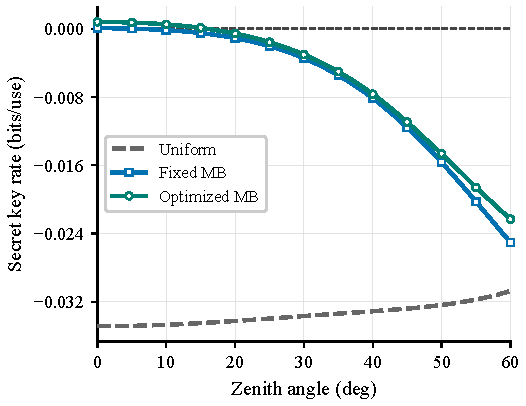
\includegraphics[width=\columnwidth]{skr_vs_zenith_publication.pdf}
  \caption{Saved raw SKR for Uniform, Fixed Maxwell--Boltzmann (MB), and Optimized MB 256-QAM over $0^\circ$--$60^\circ$, sampled every $1^\circ$. Positive samples span $0^\circ$--$5^\circ$ (Fixed MB) and $0^\circ$--$15^\circ$ (Optimized MB); Uniform remains negative. Available-catalog results are diagnostic, with incomplete source-convergence evidence for all positive rates.}
  \label{fig:skr_vs_zenith_publication}
\end{figure}

\begin{figure}[t]
  \centering
  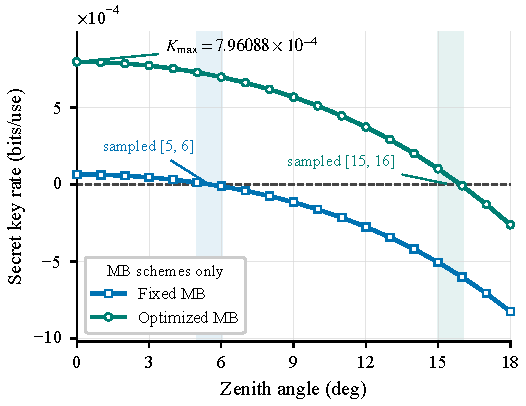
\includegraphics[width=\columnwidth]{skr_vs_zenith_zoom.pdf}
  \caption{Saved raw-SKR zoom for Fixed MB and Optimized MB over $0^\circ$--$18^\circ$ on the $1^\circ$ grid; Uniform is omitted. Positive samples span $0^\circ$--$5^\circ$ (Fixed MB) and $0^\circ$--$15^\circ$ (Optimized MB); Uniform remains negative. Shaded $[5^\circ,6^\circ]$ and $[15^\circ,16^\circ]$ intervals bracket sampled sign changes, not established continuous-angle thresholds. Available-catalog results are diagnostic, with incomplete source-convergence evidence for all positive rates.}
  \label{fig:skr_vs_zenith_zoom}
\end{figure}

\begin{figure*}[t]
  \centering
  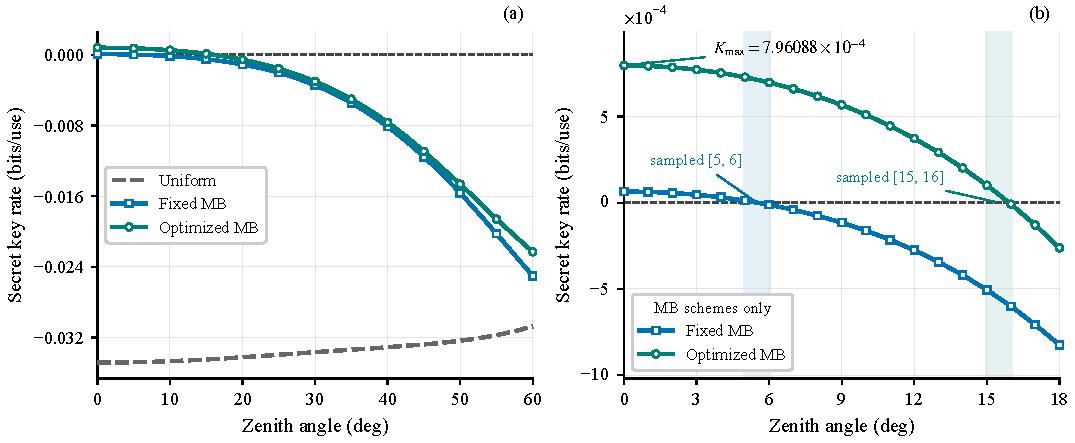
\includegraphics[width=\textwidth]{skr_vs_zenith_two_panel.pdf}
  \caption{Saved raw SKR on the $1^\circ$ grid: (a) Uniform, Fixed MB, and Optimized MB over $0^\circ$--$60^\circ$; (b) MB-only zoom over $0^\circ$--$18^\circ$. Positive samples span $0^\circ$--$5^\circ$ (Fixed MB) and $0^\circ$--$15^\circ$ (Optimized MB); Uniform remains negative. Shaded $[5^\circ,6^\circ]$ and $[15^\circ,16^\circ]$ intervals bracket sampled sign changes, not established continuous-angle thresholds. Available-catalog results are diagnostic, with incomplete source-convergence evidence for all positive rates.}
  \label{fig:skr_vs_zenith_two_panel}
\end{figure*}
